\chapter{Convolutional Neural Network}
\label{cha:CNN}


\section{Network Architecture and Initial Model}
\label{sec:initialModel}





\begin{figure}[H]
    \centering
    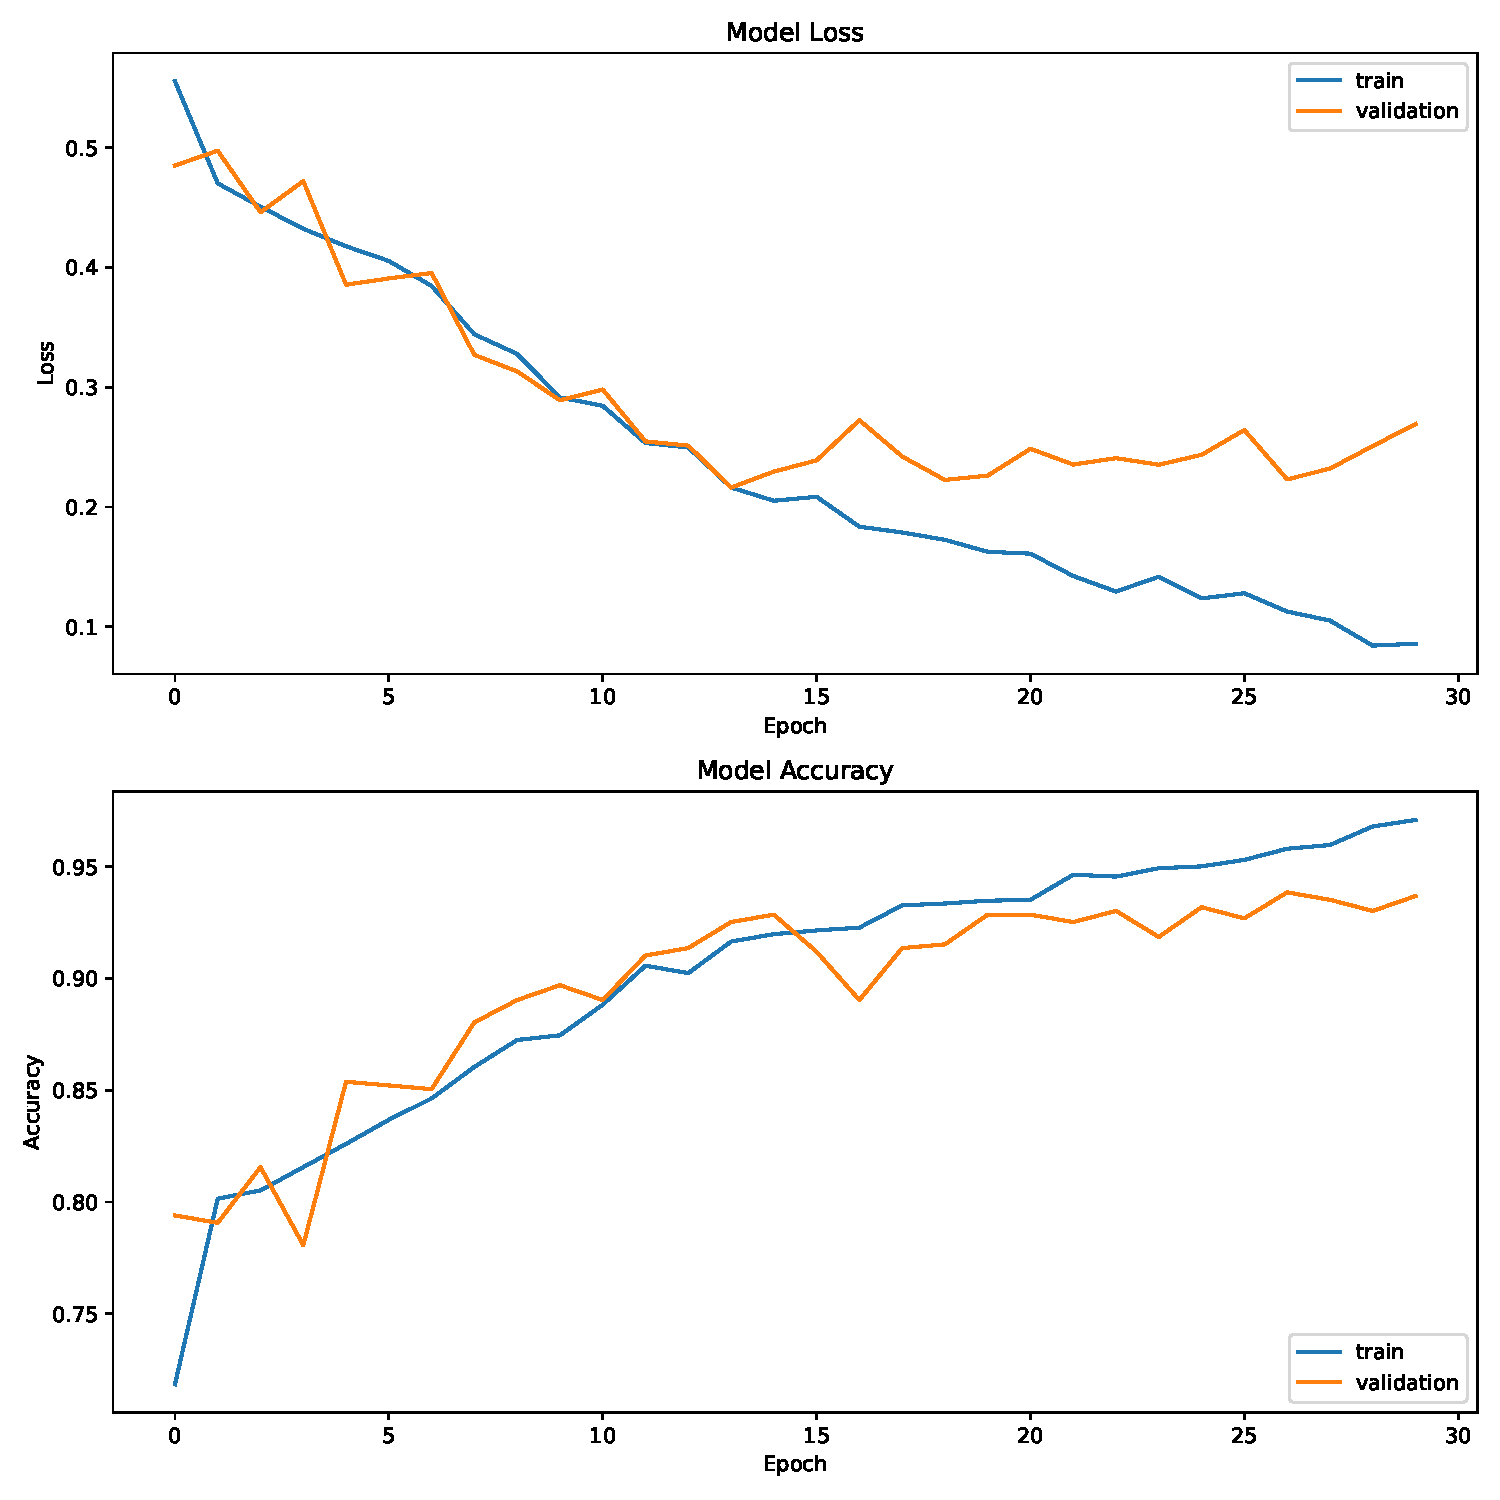
\includegraphics[width=.7\textwidth]{plots/CNN_history.pdf}
    \caption{Accuracy- and loss-curves for the initial CNN.}
    \label{fig:learningCurveInitial}
\end{figure}


\begin{figure}[H]
    \centering
    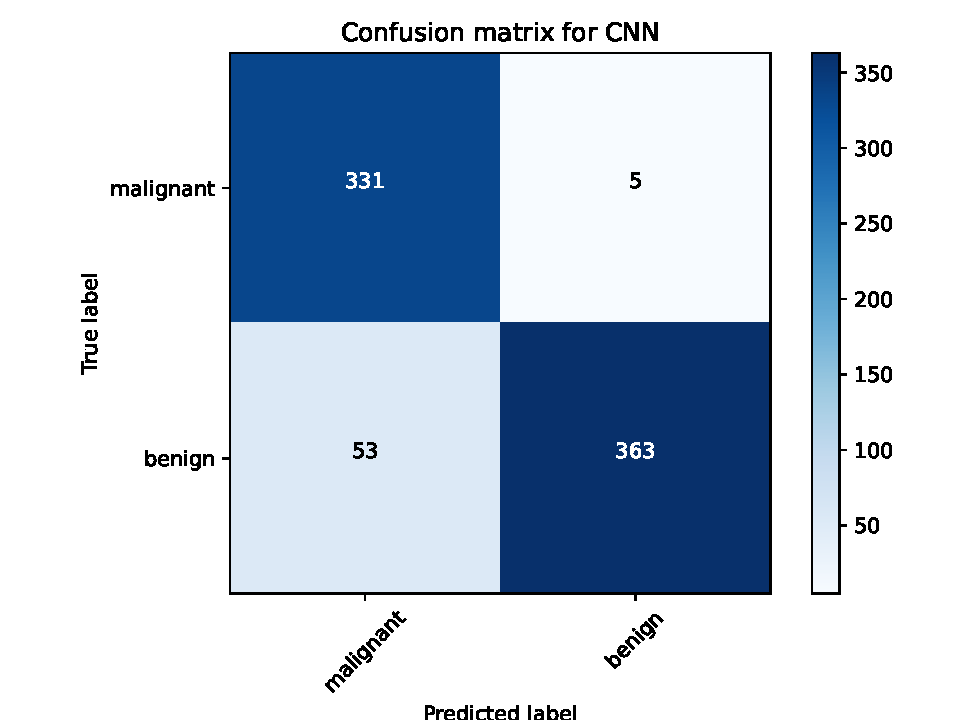
\includegraphics[width=.5\textwidth]{plots/confusion_matrix_CNN.pdf}
    \caption{Confusion matrix for the initial CNN.}
    \label{fig:confusionMatrixInitial}
\end{figure}



\section{Hyperparameter Optimization}
\label{sec:hyperparameter}



\begin{figure}[H]
    \centering
    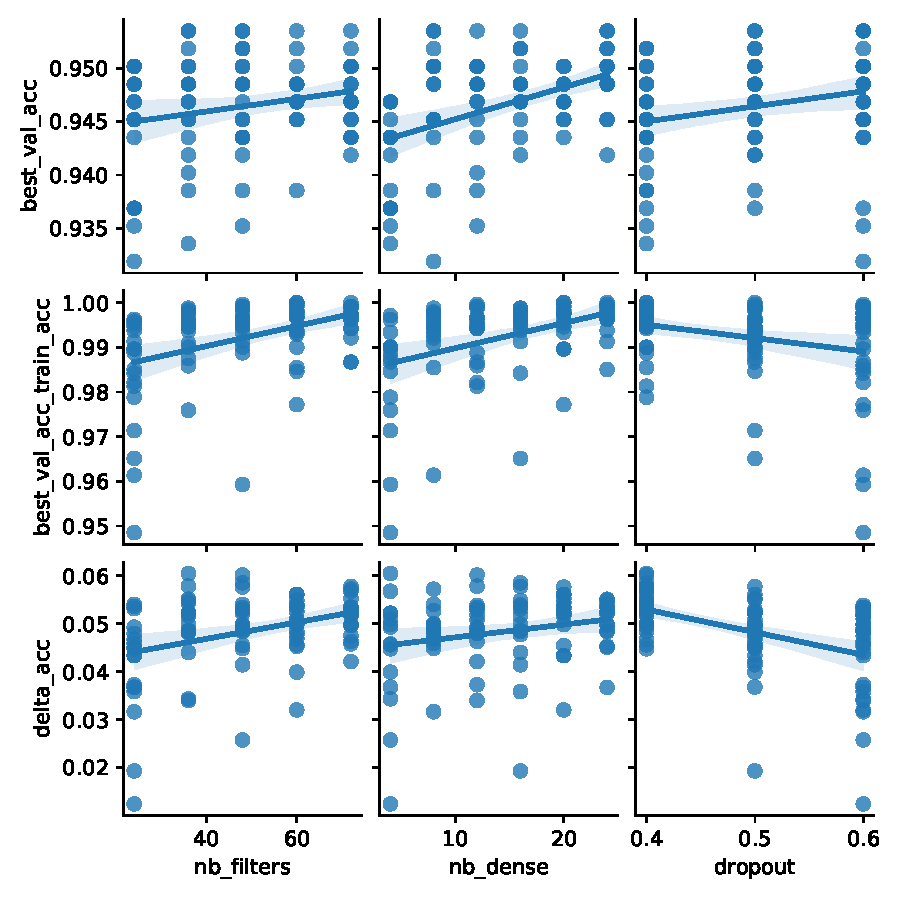
\includegraphics[width=0.7\textwidth]{plots/pairplot.pdf}
    \caption{Hyperparameter testing using gridsearch.}
    \label{fig:gridsearch}
\end{figure}

\begin{figure}[H]
    \centering
    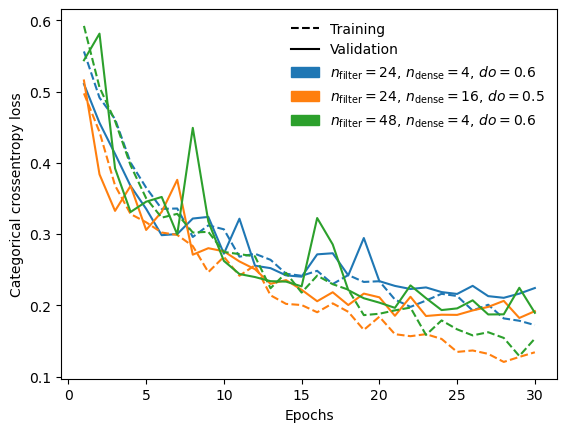
\includegraphics[width=0.7\textwidth]{plots/SmallestDelta_LearningCurves.png}
    \caption{Learning curves of the models from the gridsearch with the least difference between training and validation.}
    \label{fig:SmallestDelta_LearningCurves}
\end{figure}


\section{Final Model}
\label{sec:finalModel}

\begin{figure}[H]
    \centering
    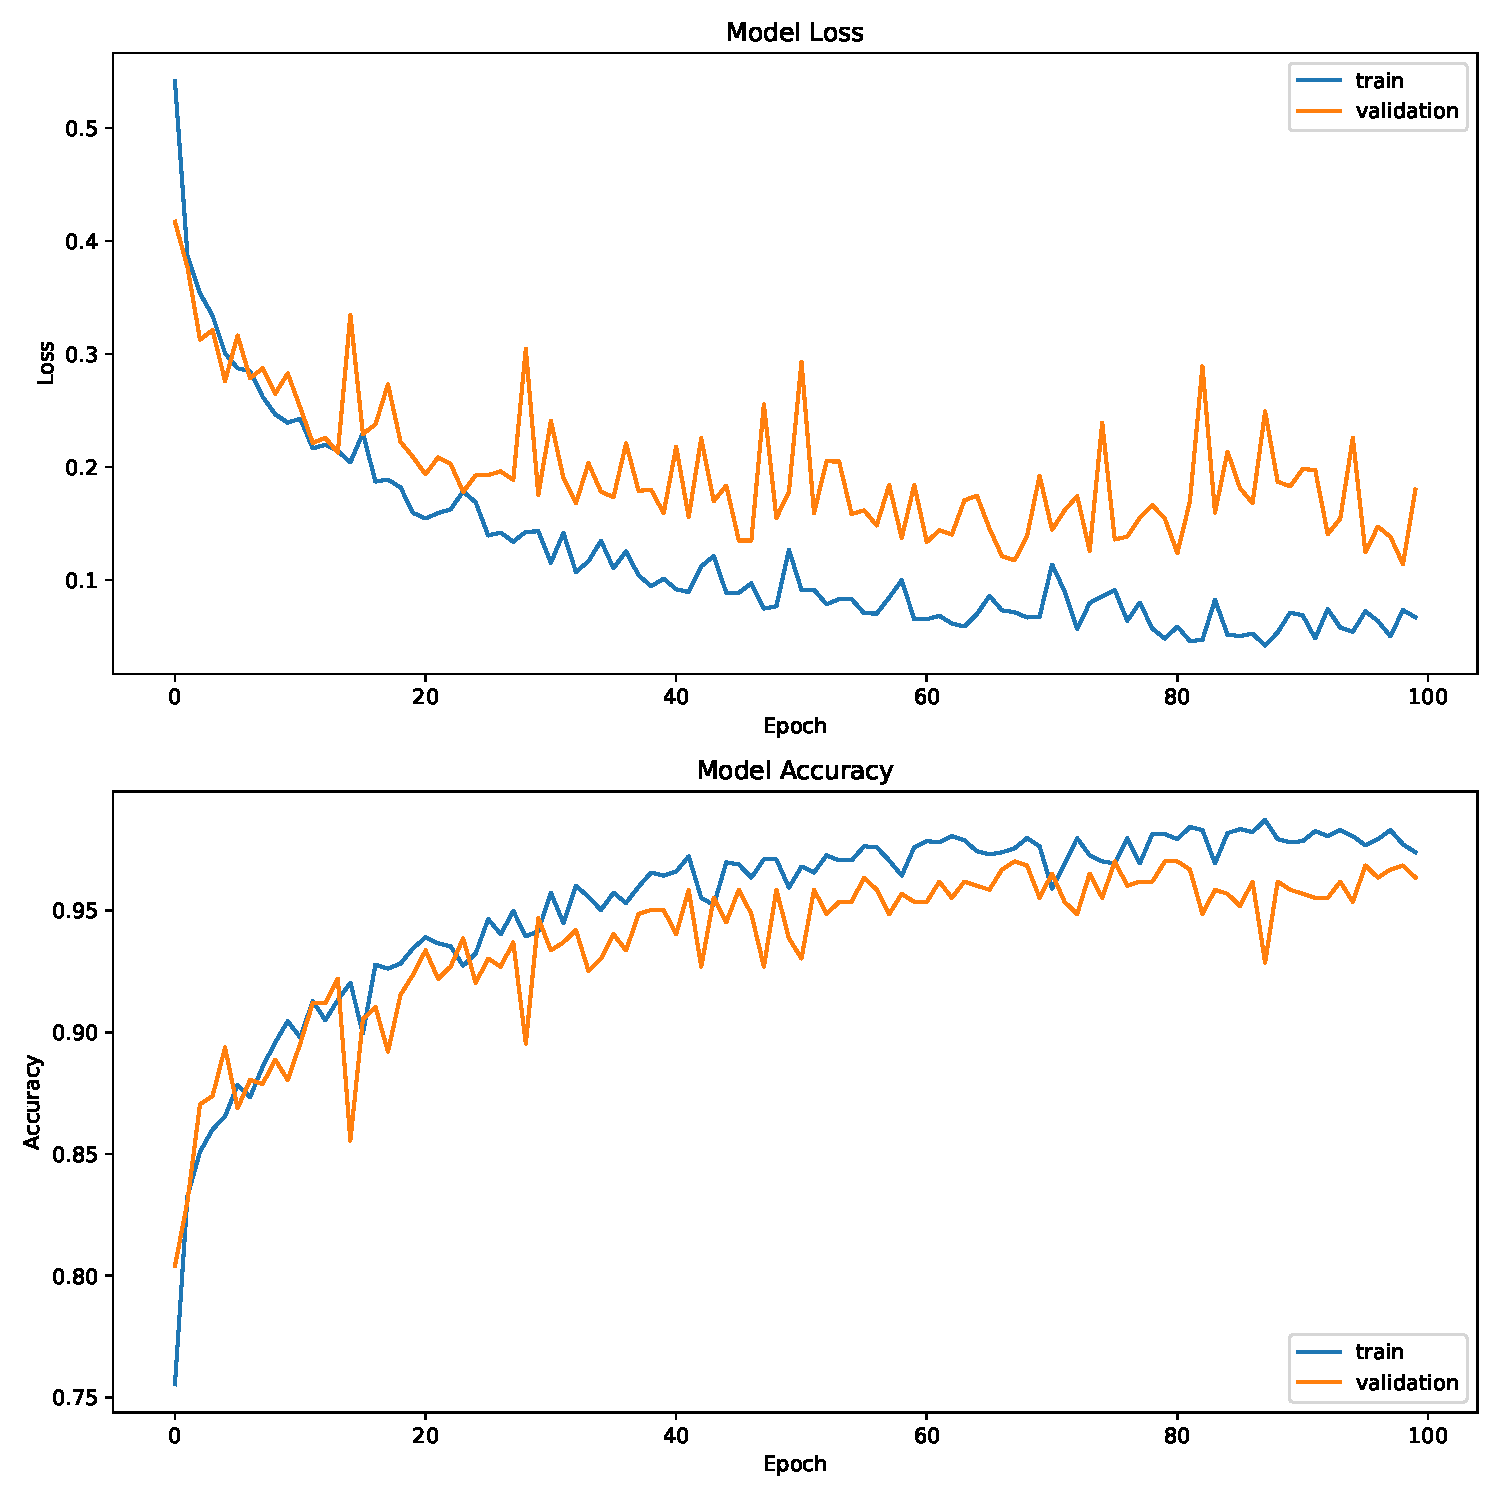
\includegraphics[width=.7\textwidth]{plots/history.pdf}
    \caption{Accuracy- and loss-curves for the initial CNN.}
    \label{fig:learningCurveFinal}
\end{figure}


\begin{figure}[H]
    \centering
    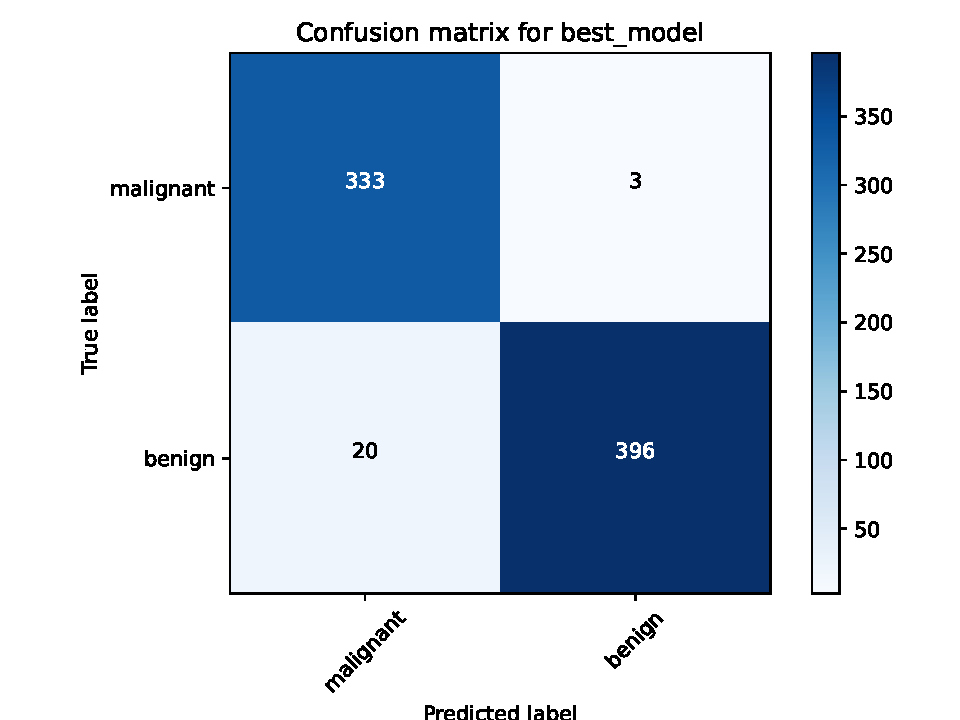
\includegraphics[width=.5\textwidth]{plots/confusion_matrix_best_model.pdf}
    \caption{Confusion matrix for the initial CNN.}
    \label{fig:confusionMatrixFinal}
\end{figure}